\documentclass[../../main.tex]{subfiles}

\usetikzlibrary{calc,trees,positioning,arrows,chains,shapes.geometric,%
    decorations.pathreplacing,decorations.pathmorphing,shapes,%
    matrix,shapes.symbols}

\tikzset{
  blockbig/.style={
    rectangle,
    draw=black, very thick,
    text width=30em,
    minimum height=3em,
    text centered,
    on chain},
  blockmedium/.style={
    rectangle,
    draw=black, very thick,
    text width=25em,
    minimum height=3em,
    text centered,
    on chain},
  blockmediumsmall/.style={
    rectangle,
    draw=black, very thick,
    text width=15em,
    minimum height=3em,
    text centered,
    on chain},
  blocksmall/.style={
    rectangle,
    draw=black, very thick,
    text width=10em,
    minimum height=3em,
    text centered},
  blocktiny/.style={
    rectangle,
    draw=black, very thick,
    text width=5em,
    minimum height=3em,
    text centered},
  every join/.style={thick},
}

\tikzstyle{line}=[draw,thick]
\tikzstyle{arrow}=[draw,thick,>=latex,->]

\begin{document}

  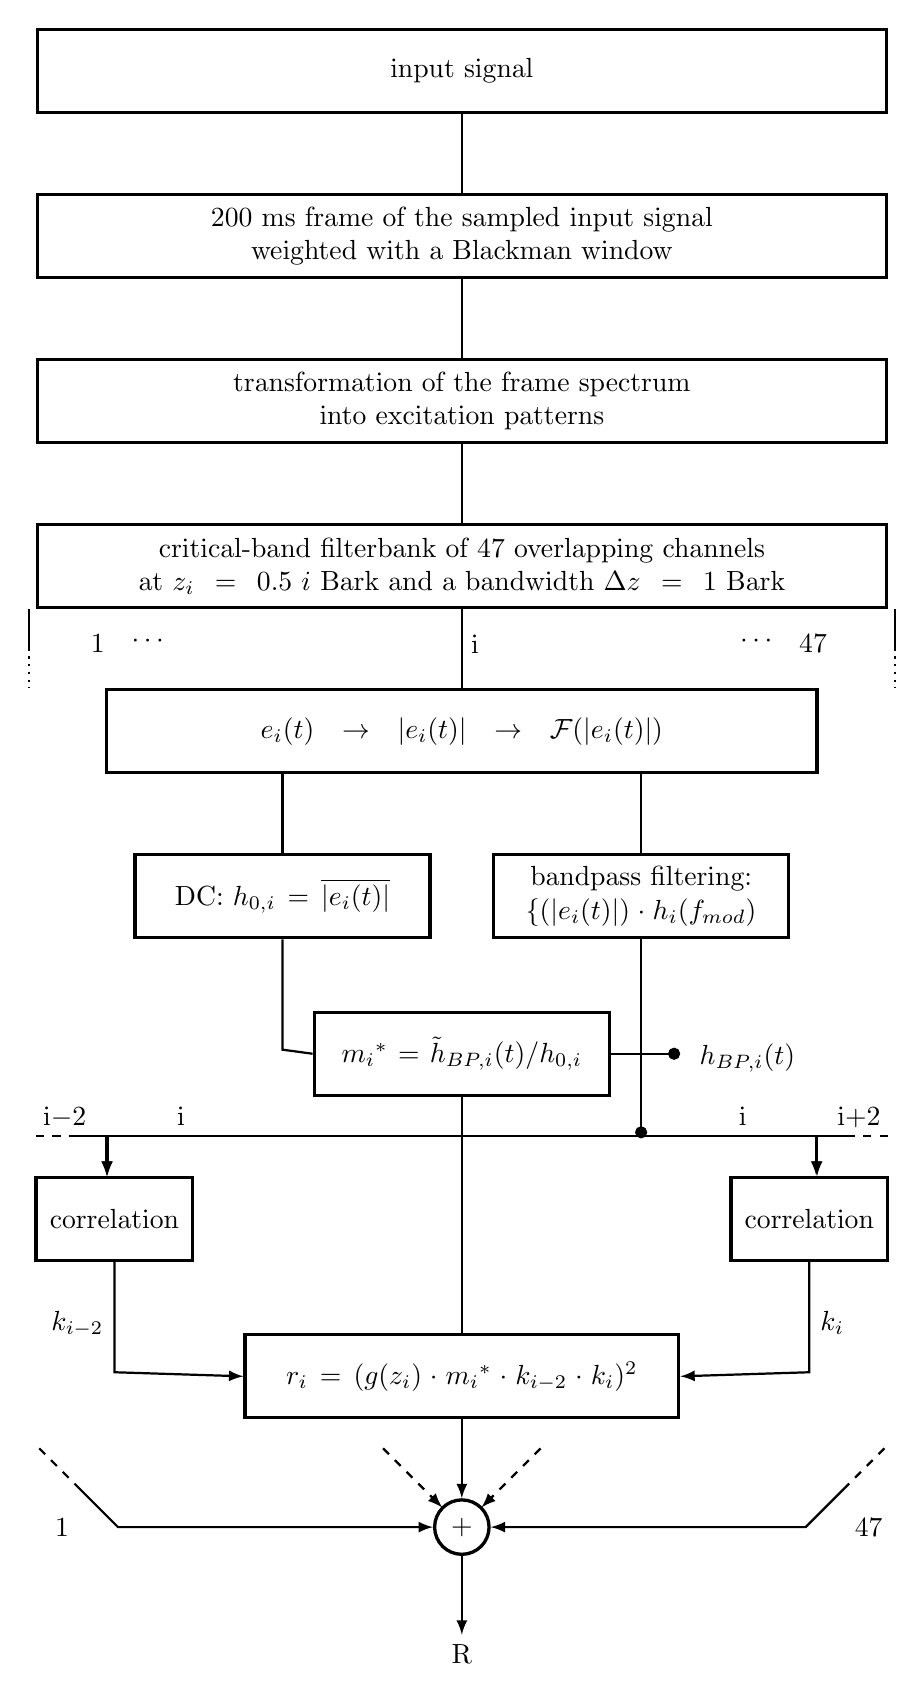
\begin{tikzpicture}
    [node distance=1cm,
    start chain=going below]

    \node[blockbig, join](input)
      {input signal};
    \node[blockbig, join](window)
      {200 ms frame of the sampled input signal\\%
      weighted with a Blackman window};
    \node[blockbig, join](patterns)
      {transformation of the frame spectrum\\into excitation patterns};
    \node[blockbig, join](filterbank)
      {critical-band filterbank of 47 overlapping channels\\%
      at $z_i = 0.5\ i$ Bark and a bandwidth $\Delta z = 1$ Bark};
    \node[blockmedium, join](fourier)
      {$e_{i}(t)\to|e_{i}(t)|\to\mathcal{F}(|e_{i}(t)|)$};
    \node[blocksmall, below left=1cm and -41.5mm of fourier](dc)
      {DC: $h_{0,i}=\overline{|e_{i}(t)|}$};
    \node[blocksmall, below right=1cm and -41.5mm of fourier](filter)
      {bandpass filtering:\\ $\mathcal{f}(|e_{i}(t)|) \cdot h_{i}(f_{mod})$};
    \node[blocksmall, below=3cm of fourier](m*)
      {${m_i}^* = \tilde{h}_{BP,i}(t)/h_{0,i}$};
    \node[blocktiny, below left=1cm and 15mm of m*](correlation_left)
      {correlation};
    \node[blocktiny, below right=1cm and 15mm of m*](correlation_right)
      {correlation};
    \node[blockmediumsmall, below=3cm of m*](ri)
      {$r_i = (g(z_i) \cdot {m_i}^* \cdot k_{i-2} \cdot k_i)^2$};
    \node[circle, draw=black, very thick, on chain](sum){+};
    \node[on chain](R){R};

    \node[below left=2mm and -5.75cm of filterbank](i){i};
    \node[below left=2mm and -1cm of filterbank](k1){1};
    \node[below left=2mm and -1.75cm of filterbank](d1){$\cdots$};
    \node[below right=2mm and -1.25cm of filterbank](k47){47};
    \node[below right=2mm and -2cm of filterbank](d2){$\cdots$};

    \node[below right=-8mm and 1cm of m*](hbpi){$h_{BP,i}(t)$};
    \node[below left=0cm and 1.5cm of m*](ic2){i};
    \node[below left=0cm and 2.75cm of m*](i-2){i$-$2};
    \node[below right=0cm and 1.5cm of m*](ic1){i};
    \node[below right=0cm and 2.75cm of m*](i+2){i+2};
    \node[below left=5mm and -10mm of correlation_left](ki-2){$k_{i-2}$};
    \node[below right=5mm and -10mm of correlation_right](ki){$k_i$};

    \node[left=4.5cm of sum](c1){1};
    \node[right=4.5cm of sum](c47){47};

    \draw[line] (filterbank.south) +(-5.5,0.0) -- +(-5.5,-0.5);
    \draw[line,dotted] (filterbank.south) +(-5.5,-0.5) -- +(-5.5,-1.0);
    \draw[line] (filterbank.south) +(5.5,0.0) -- +(5.5,-0.5);
    \draw[line,dotted] (filterbank.south) +(5.5,-0.5) -- +(5.5,-1.0);

    \draw[line] (dc.north)--(dc|-fourier.south);
    \draw[line] (filter.north)--(filter|-fourier.south);
    \draw[line] (dc.south) -- +(0.0,-1.4) -- (m*.west);
    \draw[line] (filter.south) -- +(0.0,-2.45);
    \draw[line] (m*.east) -- +(0.8,0.0);
    \draw[line] (m*.south) -- (ri.north);
    \draw[arrow] (m*.south) -- +(0.0,-0.5) -- +(-4.5,-0.5) -- +(-4.5,-1.0);
    \draw[arrow] (m*.south) -- +(0.0,-0.5) -- +(4.5,-0.5) -- +(4.5,-1.0);
    \draw[arrow] (ri.south) -- (sum.north);
    \draw[arrow] (correlation_left.south) -- +(0.0,-1.4) -- (ri.west);
    \draw[arrow] (correlation_right.south) -- +(0.0,-1.4) -- (ri.east);
    \draw[arrow] (sum.south) -- (R.north);

    \draw[line,dashed] (sum.west) +(-5.0,1.0) -- +(-4.5,0.5);
    \draw[arrow] (sum.west) +(-4.5,0.5) -- +(-4.0,0.0) -- (sum.west);
    \draw[line,dashed] (sum.east) +(5.0,1.0) -- +(4.5,0.5);
    \draw[arrow] (sum.east) +(4.5,0.5) -- +(4.0,0.0) -- (sum.east);

    \draw[arrow] (correlation_left.north) +(-0.5,0.5) -- +(-0.1,0.5) --
      +(-0.1,0.0);
    \draw[line,dashed] (correlation_left.north) +(-1.0,0.5) -- +(-0.5,0.5);
    \draw[arrow] (correlation_right.north) +(0.5,0.5) -- +(0.1,0.5) --
      +(0.1,0.0);
    \draw[line,dashed] (correlation_right.north) +(1.0,0.5) -- +(0.5,0.5);

    \draw[arrow,dashed] (sum) +(-1.0,1.0) -- +(-0.25,0.25);
    \draw[arrow,dashed] (sum) +(1.0,1.0) -- +(0.25,0.25);

    \filldraw[black] (m*.east) +(0.8,0.0) circle (2pt);
    \filldraw[black] (filter.south) +(0.0,-2.45) circle (2pt);

\end{tikzpicture}

\end{document}
